\chapter{循环}

\section{while}

\subsection{while}

在while循环中,当条件满足时重复循环体内的语句。如果条件永远为真,循环会永无止境的进行下去(死循环),因此循环体内要有改变条件的机会。\\

控制循环次数的方法就是设置循环变量:初值、判断、更新。\\

while循环的特点是先判断、再执行,所以循环体有可能会进入一次或多次,也有可能一次也不会进入。

\vspace{-0.5cm}

\begin{lstlisting}[language=Python]
while condition:
    # code
\end{lstlisting}

\vspace{0.5cm}

\mybox{计算5个人的平均身高}

\begin{lstlisting}[language=Python]
total = 0
i = 1

while i <= 5:
    height = float(input("输入第%d个人的身高:" % i))
    total += height
    i += 1

average = total / 5
print("平均身高:%.2f" % average)
\end{lstlisting}

\begin{tcolorbox}
	\mybox{运行结果}
	\begin{verbatim}
输入第1个人的身高:160.8
输入第2个人的身高:175.2
输入第3个人的身高:171.2
输入第4个人的身高:181.3
输入第5个人的身高:164
平均身高:170.5
\end{verbatim}
\end{tcolorbox}

\vspace{0.5cm}

\mybox{斐波那契数列}

\begin{figure}[H]
	\centering
	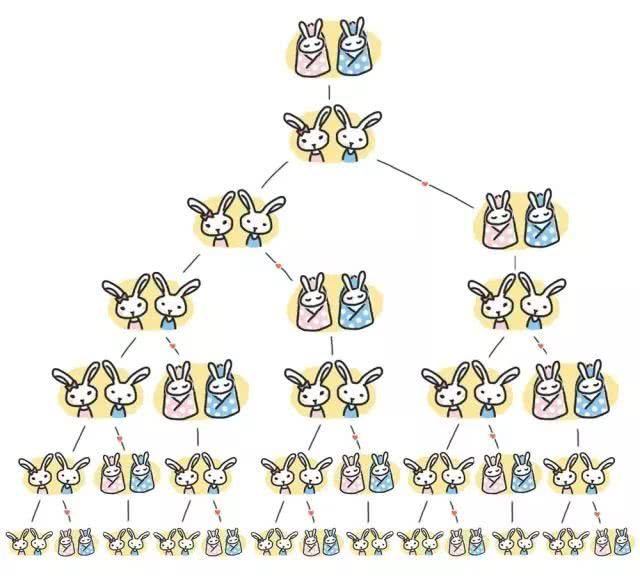
\includegraphics[scale=0.5]{img/C3/3-1/1.png}
\end{figure}

\vspace{-0.5cm}

\begin{lstlisting}[language=Python]
num1 = 0
num2 = 1
while num2 < 1000:
    print(num2, end=' ')
    num1, num2 = num2, num1 + num2
\end{lstlisting}

\begin{tcolorbox}
	\mybox{运行结果}
	\begin{verbatim}
1 1 2 3 5 8 13 21 34 55 89 144 233 377 610 987
\end{verbatim}
\end{tcolorbox}

\vspace{0.5cm}

\subsection{死循环}

对于循环的操作而言,一定要避免死循环所带来的问题。所谓的死循环指的就是循环结束条件没有得到正常的修改,导致程序无法结束。如果在执行中真的出现了死循环,命令行方式下可以直接按下Ctrl+C来中断执行。\\

\begin{figure}[H]
	\centering
	
\includegraphics[scale=0.2]{img/C3/3-1/2.png}
\end{figure}

\mybox{猜数字}

\begin{lstlisting}[language=Python]
import random           # 随机模块

answer = random.randint(1, 100)     # 产生1-100之间的随机数
cnt = 0         # 猜测次数

while True:
    num = int(input("猜一个1-100之间的数字:"))
    cnt += 1

    if num > answer:
        print("猜大了")
    elif num < answer:
        print("猜小了")
    else:       # 猜对了就跳出循环
        break

print("猜对了!你一共用了%d次猜对!" % cnt)
\end{lstlisting}

\begin{tcolorbox}
	\mybox{运行结果}
	\begin{verbatim}
猜一个1-100之间的数字:50
猜大了!
猜一个1-100之间的数字:25
猜小了!
猜一个1-100之间的数字:37
猜小了!
猜一个1-100之间的数字:43
猜小了!
猜一个1-100之间的数字:46
猜小了!
猜一个1-100之间的数字:48
猜小了!
猜一个1-100之间的数字:49
猜对了!你一共用了7次猜对!
\end{verbatim}
\end{tcolorbox}

\newpage

\section{for}

\subsection{for}

for循环的功能是在输出指定范围内的数据操作。在每一次for循环里面都会自动的获取给定范围中的每一个元素,并且在for语句里面进行相关的处理操作。\\

range()生成一个从0开始的数据范围,并且是按照线性的方式增长的。range()也可以设置数据的开始值,默认从0开始。range()的步长默认为1。\\

\mybox{for}

\begin{lstlisting}[language=Python]
for i in range(5):
    print(i, end=' ')
print()

for i in range(10, 20):
    print(i, end=' ')
print()

for i in range(1, 10, 2):
    print(i, end=' ')
print()
\end{lstlisting}

\begin{tcolorbox}
	\mybox{运行结果}
	\begin{verbatim}
0 1 2 3 4 
10 11 12 13 14 15 16 17 18 19
1 3 5 7 9
\end{verbatim}
\end{tcolorbox}

\vspace{0.5cm}

\mybox{计算1 $ \sim $ 100的累加和}

\begin{lstlisting}[language=Python]
sum = 0
for i in range(1, 101):
    sum += i
print("累加:%d" % sum)
\end{lstlisting}

\begin{tcolorbox}
	\mybox{运行结果}
	\begin{verbatim}
累加:5050
\end{verbatim}
\end{tcolorbox}

\vspace{0.5cm}

\mybox{计算$ 1 + {1 \over 2} + {1 \over 3} + ... + {1 \over n} $}

\begin{lstlisting}[language=Python]
sum = 0
n = int(input("输入n:"))

for i in range(1, n+1):
    sum += 1 / i
print(sum)
\end{lstlisting}

\begin{tcolorbox}
	\mybox{运行结果}
	\begin{verbatim}
输入n:10
2.9289682539682538
\end{verbatim}
\end{tcolorbox}

for循环主要是通过序列的形式完成的范围设置,而字符串也属于序列。\\

单个的字符是一种特殊的类型,是用单引号表示字符字面量。每一个字符都有其对应的码值。\\

ASCII全称American Standard Code for Information Interchange(美国信息交换标准代码),一共定义了128个字符。

\begin{longtable}{|c|c|c|c|c|c|c|c|}
	\hline
	\textbf{ASCII} & \textbf{字符} & \textbf{ASCII} & \textbf{字符} & \textbf{ASCII} & \textbf{字符}          & \textbf{ASCII} & \textbf{字符}          \\
	\hline
	0              & NUT           & 32             & (space)       & 64             & @                      & 96             & \lstinline|`| \\
	\hline
	1              & SOH           & 33             & !             & 65             & A                      & 97             & a                      \\
	\hline
	2              & STX           & 34             & \text{"}      & 66             & B                      & 98             & b                      \\
	\hline
	3              & ETX           & 35             & \#            & 67             & C                      & 99             & c                      \\
	\hline
	4              & EOT           & 36             & \$            & 68             & D                      & 100            & d                      \\
	\hline
	5              & ENQ           & 37             & \%            & 69             & E                      & 101            & e                      \\
	\hline
	6              & ACK           & 38             & \&            & 70             & F                      & 102            & f                      \\
	\hline
	7              & BEL           & 39             & \text{'}      & 71             & G                      & 103            & g                      \\
	\hline
	8              & BS            & 40             & (             & 72             & H                      & 104            & h                      \\
	\hline
	9              & HT            & 41             & )             & 73             & I                      & 105            & i                      \\
	\hline
	10             & LF            & 42             & *             & 74             & J                      & 106            & j                      \\
	\hline
	11             & VT            & 43             & +             & 75             & K                      & 107            & k                      \\
	\hline
	12             & FF            & 44             & ,             & 76             & L                      & 108            & l                      \\
	\hline
	13             & CR            & 45             & -             & 77             & M                      & 109            & m                      \\
	\hline
	14             & SO            & 46             & .             & 78             & N                      & 110            & n                      \\
	\hline
	15             & SI            & 47             & /             & 79             & O                      & 111            & o                      \\
	\hline
	16             & DLE           & 48             & 0             & 80             & P                      & 112            & p                      \\
	\hline
	17             & DC1           & 49             & 1             & 81             & Q                      & 113            & q                      \\
	\hline
	18             & DC2           & 50             & 2             & 82             & R                      & 114            & r                      \\
	\hline
	19             & DC3           & 51             & 3             & 83             & S                      & 115            & s                      \\
	\hline
	20             & DC4           & 52             & 4             & 84             & T                      & 116            & t                      \\
	\hline
	21             & NAK           & 53             & 5             & 85             & U                      & 117            & u                      \\
	\hline
	22             & SYN           & 54             & 6             & 86             & V                      & 118            & v                      \\
	\hline
	23             & TB            & 55             & 7             & 87             & W                      & 119            & w                      \\
	\hline
	24             & CAN           & 56             & 8             & 88             & X                      & 120            & x                      \\
	\hline
	25             & EM            & 57             & 9             & 89             & Y                      & 121            & y                      \\
	\hline
	26             & SUB           & 58             & :             & 90             & Z                      & 122            & z                      \\
	\hline
	27             & ESC           & 59             & ;             & 91             & [                      & 123            & \{                     \\
			\hline
	28             & FS            & 60             & <             & 92             & /                      & 124            & |                      \\
			\hline
	29             & GS            & 61             & =             & 93             & ]                      & 125            & \}                     \\
	\hline
	30             & RS            & 62             & >             & 94             & \lstinline|^| & 126            & \lstinline|~| \\
	\hline
	31             & US            & 63             & ?             & 95             & \_                     & 127            & DEL                    \\
	\hline
	\caption{ASCII码表}
\end{longtable}

\vspace{-0.5cm}

\mybox{小写字母转大写}

\begin{lstlisting}[language=Python]
str = "Hello World!"

for s in str:
    # 小写字母
    if 97 <= ord(s) <= 122:     # ord():字符转ASCII码
        s = chr(ord(s) - 32)    # chr():ASCII码转字符
    print(s, end='')
\end{lstlisting}

\begin{tcolorbox}
	\mybox{运行结果}
	\begin{verbatim}
HELLO WORLD!
\end{verbatim}
\end{tcolorbox}

\vspace{0.5cm}

\subsection{嵌套循环}

循环也可以进行嵌套使用。\\

\mybox{九九乘法表}\\

\begin{table}[H]
	\centering
	\setlength{\tabcolsep}{1.5mm}{
		\begin{tabular}{|c|c|c|c|c|c|c|c|c|}
			\hline
			1*1=1 & 1*2=2  & 1*3=3  & 1*4=4  & 1*5=5  & 1*6=6  & 1*7=7  & 1*8=8  & 1*9=9  \\
			\hline
			2*1=2 & 2*2=4  & 2*3=6  & 2*4=8  & 2*5=10 & 2*6=12 & 2*7=14 & 2*8=16 & 2*9=18 \\
			\hline
			3*1=3 & 3*2=6  & 3*3=9  & 3*4=12 & 3*5=15 & 3*6=18 & 3*7=21 & 3*8=24 & 3*9=27 \\
			\hline
			4*1=4 & 4*2=8  & 4*3=12 & 4*4=16 & 4*5=20 & 4*6=24 & 4*7=28 & 4*8=32 & 4*9=36 \\
			\hline
			5*1=5 & 5*2=10 & 5*3=15 & 5*4=20 & 5*5=25 & 5*6=30 & 5*7=35 & 5*8=40 & 5*9=45 \\
			\hline
			6*1=6 & 6*2=12 & 6*3=18 & 6*4=24 & 6*5=30 & 6*6=36 & 6*7=42 & 6*8=48 & 6*9=54 \\
			\hline
			7*1=7 & 7*2=14 & 7*3=21 & 7*4=28 & 7*5=35 & 7*6=42 & 7*7=49 & 7*8=56 & 7*9=63 \\
			\hline
			8*1=8 & 8*2=16 & 8*3=24 & 8*4=32 & 8*5=40 & 8*6=48 & 8*7=56 & 8*8=64 & 8*9=72 \\
			\hline
			9*1=9 & 9*2=18 & 9*3=27 & 9*4=36 & 9*5=45 & 9*6=54 & 9*7=63 & 9*8=72 & 9*9=81 \\
			\hline
		\end{tabular}
	}
	\caption{九九乘法表}
\end{table}

\begin{lstlisting}[language=Python]
for i in range(1, 10):
    for j in range(1, 10):
        print("%d*%d=%d" % (i, j, i*j), end='\t')
    print()
\end{lstlisting}

\vspace{0.5cm}

\mybox{输出图案}

\begin{lstlisting}
*
**
***
****
*****
\end{lstlisting}

\begin{lstlisting}[language=Python]
for i in range(5):
    for j in range(i+1):
        print("*", end='')
    print()
\end{lstlisting}

\newpage

\section{break or continue?}

\subsection{循环控制}

循环控制语句的作用是控制当前的循环结构是否继续向下执行,如果不进行控制,那么会根据既定的结构重复执行。如果有一些特殊的情况导致循环的执行中断,就称为循环的控制语句。循环控制语句的关键字有break和continue。\\

break的作用是跳出当前循环,执行当前循环之后的语句。break只能跳出一层循环,如果是嵌套循环,那么需要按照嵌套的层次,逐步使用break来跳出。break语句只能在循环体内和switch语句内使用。\\

continue的作用是跳过本轮循环,开始下一轮循环的条件判断。continue终止当前轮的循环过程,但它并不跳出循环。\\

\mybox{break}

\begin{lstlisting}[language=Python]
for i in range(10):
    if i == 5:
        break
    print(i, end=' ')
\end{lstlisting}

\begin{tcolorbox}
	\mybox{运行结果}
	\begin{verbatim}
1 2 3 4
\end{verbatim}
\end{tcolorbox}

\vspace{0.5cm}

\mybox{continue}

\begin{lstlisting}[language=Python]
for i in range(10):
    if i == 5:
        continue
    print(i, end=' ')
\end{lstlisting}

\begin{tcolorbox}
	\mybox{运行结果}
	\begin{verbatim}
1 2 3 4 6 7 8 9 10
\end{verbatim}
\end{tcolorbox}

\newpage